\documentclass[10pt,letterpaper]{article}
\usepackage[top=1in,bottom=1in,left=1in,right=1in]{geometry}
\usepackage{datetime}
\usepackage{natbib}      % http://merkel.zoneo.net/Latex/natbib.php
\usepackage{palatino}
\usepackage{verbatim}
\usepackage[normalem]{ulem}
\bibpunct{(}{)}{;}{a}{,}{,}

\usepackage{array}

\usepackage{chngpage}
\usepackage{stmaryrd}
\usepackage{amssymb}
\usepackage{amsmath}
\usepackage{graphicx}
\usepackage{lscape}
\usepackage{subfigure}
\usepackage[usenames,dvipsnames]{color}
\definecolor{myblue}{rgb}{0,0.1,0.6}
\definecolor{mygreen}{rgb}{0,0.3,0.1}
\usepackage[colorlinks=true,linkcolor=black,citecolor=mygreen,urlcolor=myblue]{hyperref}

\newcommand{\bocomment}[1]{\textcolor{Bittersweet}{BO says: #1}}

\newcommand{\ignore}[1]{}
\newcommand{\transpose}{^\mathsf{T}}
\newcommand{\inner}[1]{\langle #1 \rangle} 
\newcommand{\smallsec}[1]{\noindent \textbf{#1\ }}
\newcommand{\cmd}[1] {{\color{blue}\texttt{#1}}}

\newcommand{\solution}[1]{{\color{myblue} \emph{[Solution:} 

#1 

\emph{End solution]}}}
\newcommand{\solutionnote}[1]{{\color{myblue} \emph{[Note:}

#1 

\emph{End note]}}}
\newcommand{\points}[1]{{\color{mygreen}\emph{[#1]\ \ }}}

\newcommand{\aone}{\diamondsuit}
\newcommand{\atwo}{\heartsuit}
\newcommand{\bone}{\triangle}
\newcommand{\btwo}{\Box}
\newcommand{\myand}{\ \land\ }
\newcommand{\myor}{\ \lor\ }
\newcommand{\mynot}{\lnot}

\title{
	Mini-project 4\\
	\Large{COMPSCI 370, Spring 2021, UMass Amherst} \\
	\Large{Instructor: Subhransu Maji} \\
	\Large{TAs: Chenyun Wu, Jong-Chyi Su}
}


\settimeformat{ampmtime}
\date{}

\begin{document}

\maketitle

\renewcommand\thesubsection{\thesection.\alph{subsection}}
\section*{Guidelines}
\paragraph{Submission.} Submit a \emph{single pdf} file via
Gradescope that includes your solutions, figures, and code. The latex
source file for the homework is provided in case you want to modify it
to produce your report. However, you are welcome to use other
typesetting software as long as the final output is a pdf.
For readability you may attach the code printouts at the end of the
solutions within the same pdf.
Similarly figures enable easy comparision of various approaches.
Poorly written or formatted reports will make it harder for us to
evaluate it and may lead to a deduction of credit.


\paragraph{Late policy.}
\begin{itemize}
\item You can use 7 late days, with up to 3 late days per assignment.
\item Once you have used all 7 late days, penalty is 25\% for each additional late day.
\item We will use your latest submission for grading and for calculating your late day usage.
\item There is no bonus if you don't use late days at all.
\end{itemize}


\paragraph{Plagiarism.}
We expect the students not to copy, refer to, or look at the solutions
in preparing their answers. We expect students to want to learn and
not google for answers. See the Universities' guidelines on academic
honesty (\url{https://www.umass.edu/honesty}).
Finally, we also ask you to not post the solutions online as the
problem sets might be used in future.


\paragraph{Collaboration.} The homework must be done individually,
except where otherwise noted in the assignments. 'Individually' means
each student must hand in their own answers, and each student must
write their own code in the programming part of the assignment. It is
acceptable, however, for students to collaborate in figuring out
answers and helping each other solve the problems, for example within
a study group.
We will be assuming that you will be taking the responsibility to make
sure you personally understand the solution to any work arising from
such a collaboration.


\paragraph{Python requirements.}
Our code is tested on Python 3.
The Python code depends on external
packages such as \cmd{scipy}, \cmd{numpy}, and \cmd{scikit-image}.
Take a look at the resources posted on the course page to set up the
appropriate programming environment and tutorial on basic concepts.


\paragraph{Using other programming languages.}
While we have made the starter code available in Python, 
feel free to implement the homework from scratch using your favorite
programming language. For example you are welcome to use Matlab, C, Java,
Octave or Julia, with the caveat that we may be able help you with
debugging.








\newpage


\section{Image Gradient and Orientation Histogram [15 points]}
Write a function to compute the gradient magnitude and angle (orientation) for
each pixel in an image. 
The function \cmd{imageGradient}
should take a grayscale image \cmd{im} and return two arrays, m and a,
that indicate the magnitude and angle of the gradient at each pixel in
the image. The arrays m and a should be of the same size of the image.

Note that the gradient of the image $gx$ and $gy$ can be obtained by
filtering the image with derivative filters. In this homework compute
the gradients using the following filters
$fx = [-1~0~1]$ and $fy = [-1~ 0 ~1]^T$.
The gradient magnitude is given by $m = \sqrt{gx^2 + gy^2}$ and the angle
$\theta = \tan^{-1}(gy/gx)$. In this case the angle $\theta \in
[-\pi/2,\pi/2]$ radians or $[-90, 90]$ degrees.

It is important to treat the boundary of the images carefully.
The simplest way is to pad the image using the option ``replicate''
where you repeat the sides for padding.
Padding with zeros will most certainly add a strong gradient
along the four sides.
Alternatively, you can zero out the gradient responses for pixels that
are near the boundary after computing gradients with
zero padding.

\begin{itemize}
\item \emph{(5 points)} Use your implementation to compute the
  gradient magnitude and
  angle on the \cmd{parrot.jpg} image included in the data directory (Figure~\ref{fig:parrot}). 
  Convert this image to grayscale and double format before
  applying the image filters.
  Visualize the magnitude as a grayscale
  image and angle image using the ``viridis'' colormap. This is the
  default colormap for matplotlib. See an example in
  Figure~\ref{fig:butterfly}.
\item \emph{(5 points)}
  Recompute the the above quantities by first applying a Gaussian
  filter of
  $\sigma=2$ pixels to the image.
  Display that gradient magnitude and orientation for the smoothed
  image. How is the gradient magnitude affected by smoothing?
\item \emph{(5 points)}
  Visualize the distribution of angles by computing a
  histogram of orientations as follows:
  \begin{enumerate}
    \item Bin the range of
      angles between [-90 90] degrees into 9 equal sized bins. 
  For example the first bin corresponds to angles [-90 -70) degrees
    \footnote{The notation means that -90 is included and -70 is excluded}, the
    second bin corresponds to angles [-70 -50), till 
    the last bin that corresponds to angles [70 90]. 
    \item Assign each pixel to a bin based on the angle. For example
      the angle -85.2 degrees gets assigned to bin 1, while angle 0 degrees gets
      assigned to bin 5. This step gives you a number between 1 to 9 for each pixel.
    \item For each bin compute the total magnitude by summing the magnitudes of
      all the pixels that belong to the bin. This gives you
      9 numbers that indicates the total magnitude in 9 different orientation. Weighing by the magnitude reduces the contributions of the flat regions in the image where the magnitude is close to zero and the angle is unreliable.
	  Plot the orientation histogram for this image with and without
  smoothing using a "bar" plot. See Figure~\ref{fig:butterfly}.

  \end{enumerate}
\end{itemize}

Figure~\ref{fig:butterfly} shows the gradients for the
butterfly image included in the data directory.

\begin{figure}[h]
\centering
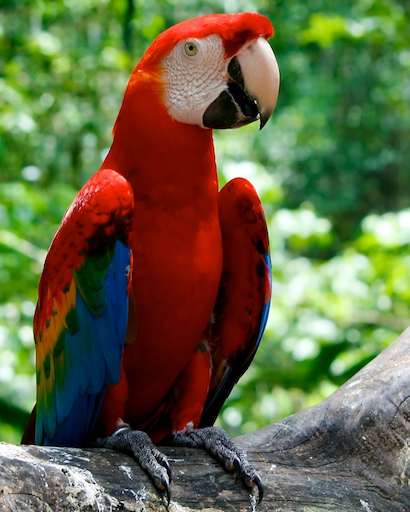
\includegraphics[width=0.2\linewidth]{figs/parrot.jpg}
\caption{\label{fig:parrot} Compute the gradient magnitude, angle, and gradient histogram for the ``parrot" image.}
\end{figure}

\begin{figure}[h]
\centering
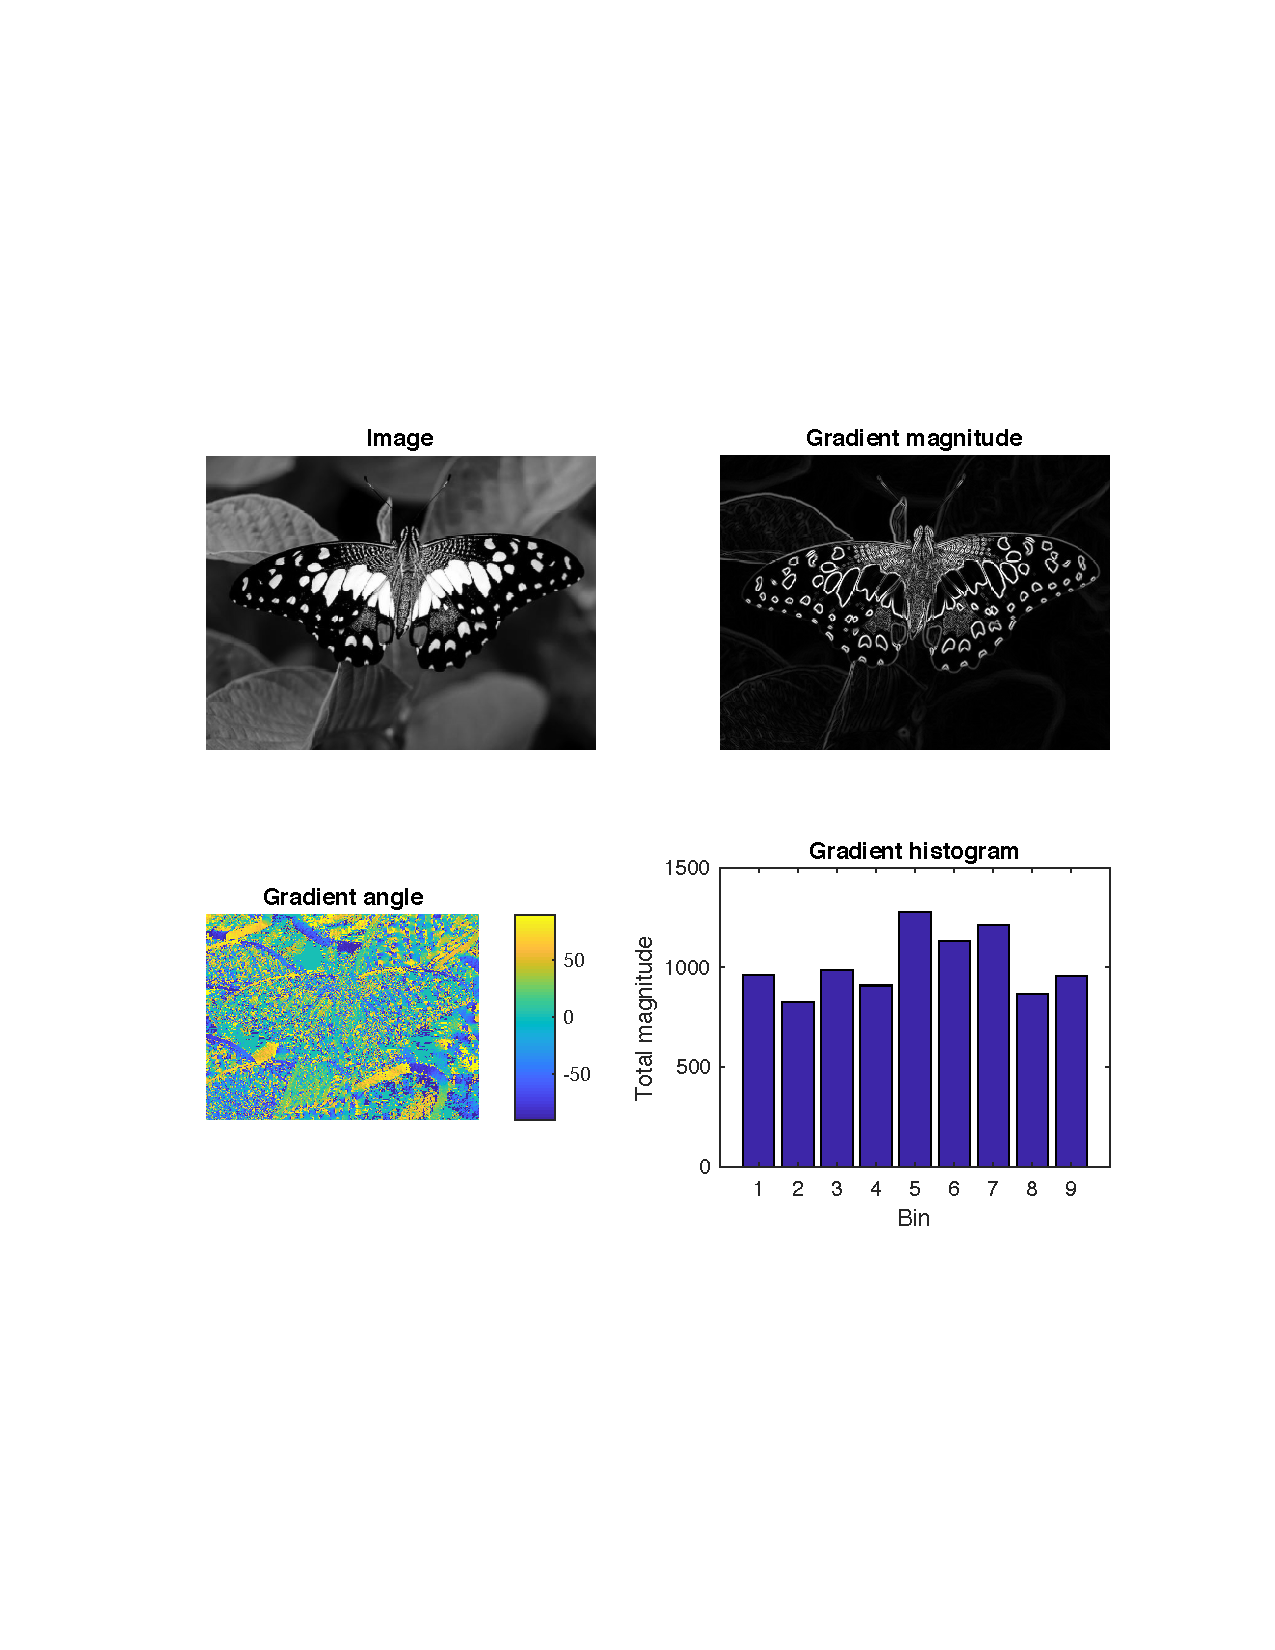
\includegraphics[width=0.8\linewidth]{figs/butterfly-result.pdf}
\vspace{-0.2in}
\caption{\label{fig:butterfly} Gradient magnitude, angle and gradient histogram for the
  butterfly image.}
\end{figure}


  

\newpage
\section{Corner Detection}
In this part you will implement two corner detection techniques as discussed in class. The first is a ``simple corner detector" that is based on how much a patch changes when you move in eight different directions. The second is the Harris corner detector which is a more accurate way of measuring the same change. Recall that the steps for detecting corners are:
\begin{enumerate}
\item Compute a per-pixel ``cornerness" score.
\item Threshold the score and compute peaks of the score (or non-maximum suppression).
\end{enumerate}

The codebase contains an implementation of Step 2. Your will implement Step 1. The entry code for this part is in \cmd{testCornerDetector}. The code loads a checkerboard image and calls the \cmd{detectCorners} function with \cmd{isSimple=true} and \cmd{isSimple=false}, and diplays the detected corners. If you run this code you should see the output in Figure~\ref{fig:checker}-top. Once you implement the corner detectors described in the next two sections the corners should be correctly detected as shown in Figure~\ref{fig:checker}-bottom.


\begin{figure}[h]
\centering
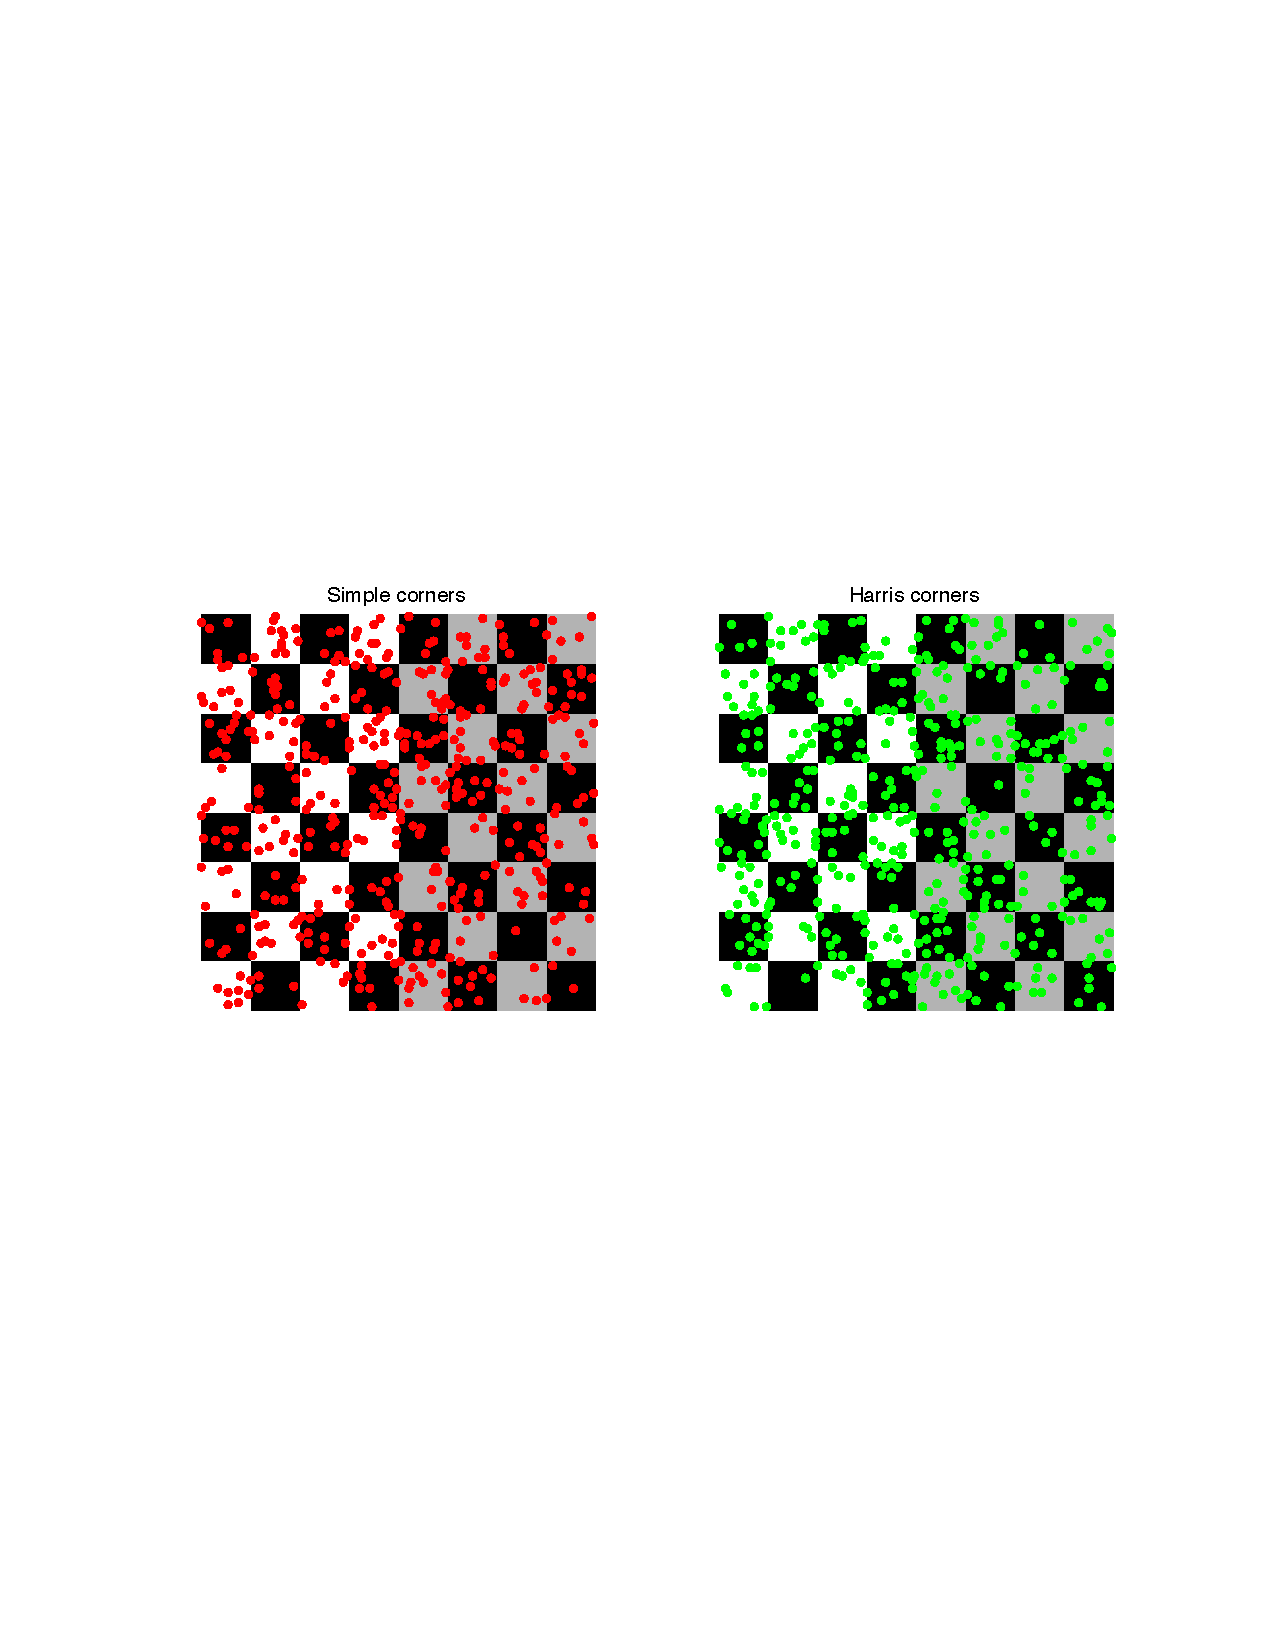
\includegraphics[width=0.75\linewidth]{figs/checkerInit.pdf} \\
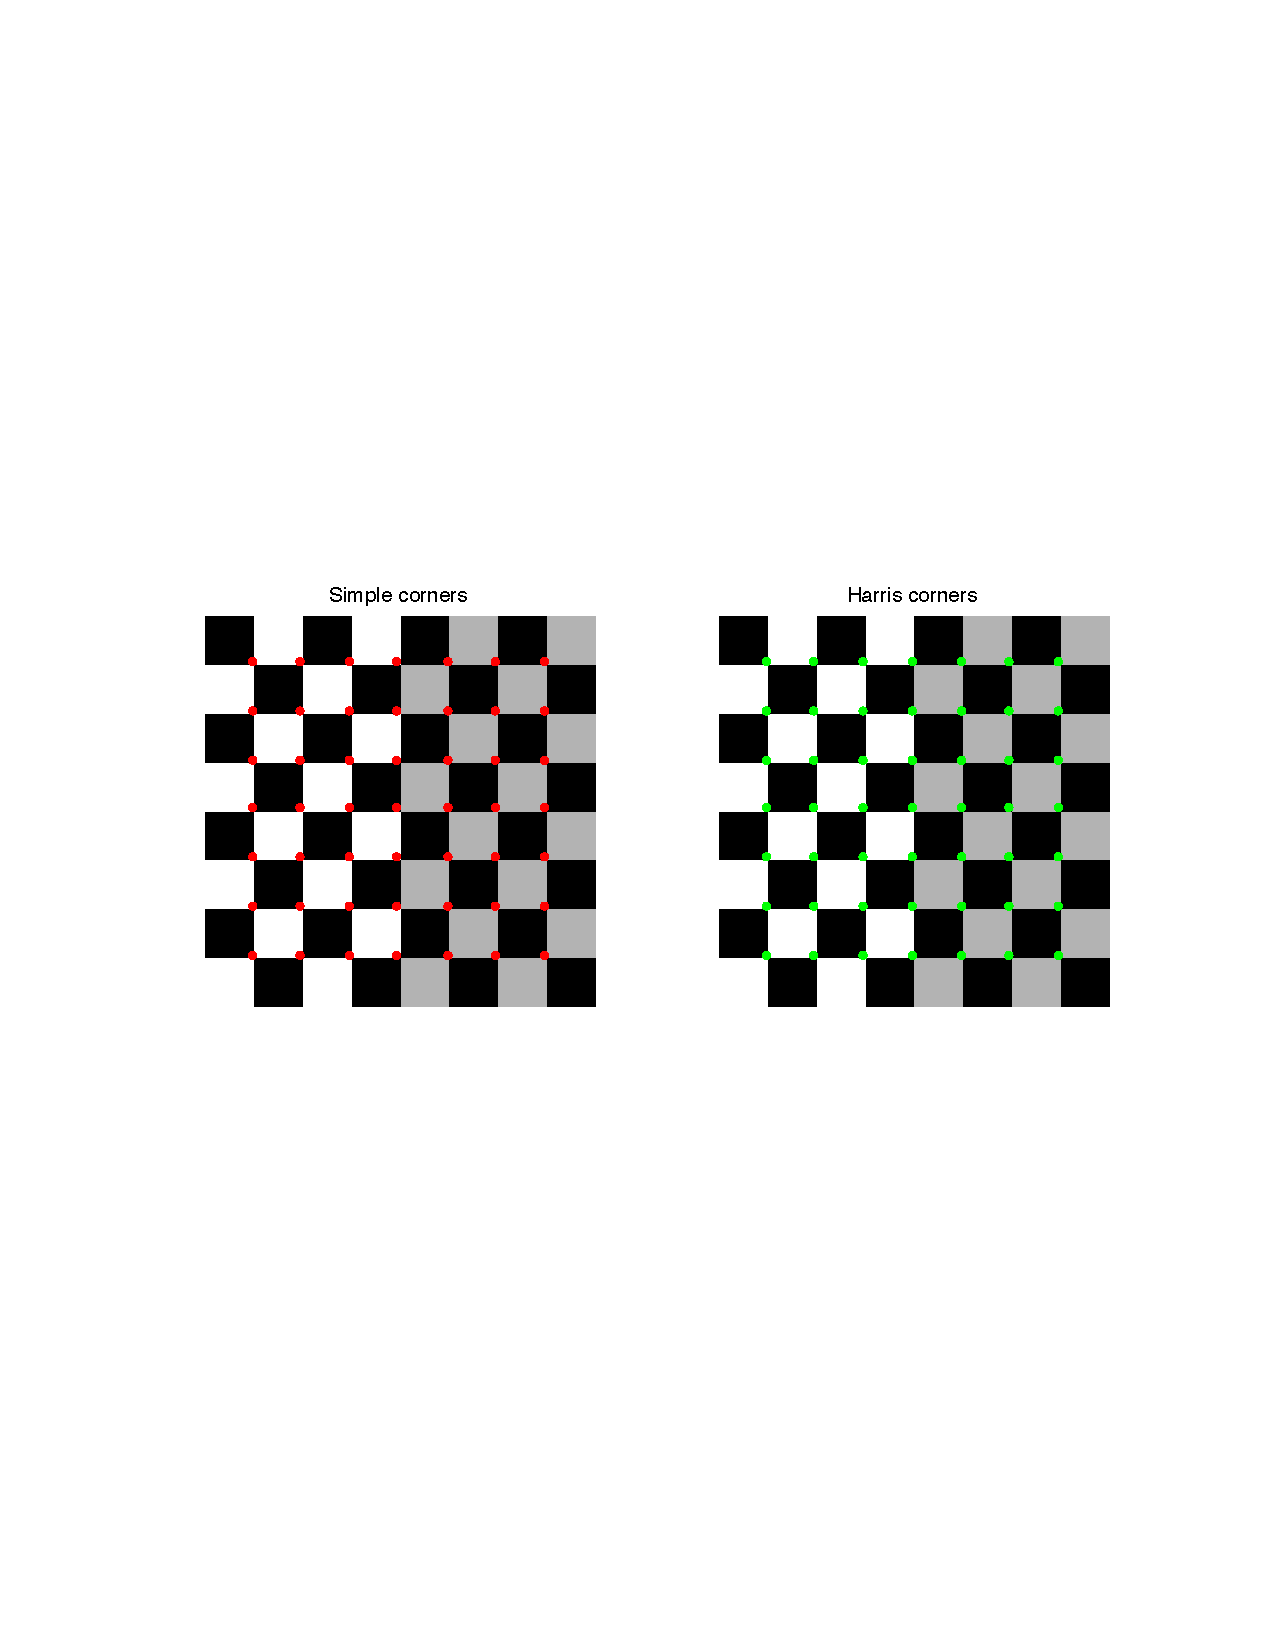
\includegraphics[width=0.75\linewidth]{figs/checkerSolution.pdf}
\caption{\label{fig:checker} \textbf{(Top)} Initial output of \cmd{testCornerDetector}. \textbf{(Bottom)} Output after the correct implementation of \cmd{detectCorners}.}
\end{figure}

Take a look inside the file \cmd{detectCorners} which now contains a
dummy implementation of the two corner detectors. Both these currently
return a
\cmd{cornerScore} image indicating how corner-like each pixel is.
This is thresholded and non-maximum suppressed to produce the
location of peaks. 
Sorting these locations by score produces the
ranked list of corner locations. If you are curious take a look at the
\cmd{nms} function.
You will replace the detectCorners with your own implementation.


\subsection{A simple corner detector [25 points]}
Recall, that the simple corner detector computes the \cmd{cornerScore} by computing the weighted sum-of-squared differences between pixels within a window and its shifted version in eight possible directions. The parameter $\cmd{w}$ specifies the $\sigma$ of the Gaussian used to compute the weighting kernel.


Implement the function \cmd{detectCorners(I, isSimple=true, w, th)}. It returns a list of x-coordinate, y-coordinate, and corner score of the corners sorted in the decreasing order of their scores. w is the window size, and th is a user-specified threshold.

You can do this by implementing the helper function \cmd{simpleScore(I, w)} inside the file, which returns \cmd{cornerScore}, an image with per-pixel scores. Right now it simply returns a random score for each pixel. The basic algorithm is to compute
\[
	E(u,v) = \left( I * f(u,v) \right)^2 * G_\sigma,
\]
for each of the eight possible shifts $(u,v)$. Here $f(u,v)$ is the filter corresponding to the difference between pixel at the center and pixel at $(u,v)$, $(\cdot)^2$ is the \emph{element-wise squaring} operation\footnote{Note the difference between element-wise squaring and matrix squaring in Python}, and $G_\sigma$ is a Gaussian kernel with standard deviation $\sigma$. The \cmd{cornerScore} is the sum of $E(u,v)$ across all of $(u,v)$, i.e., 
\[
\text{cornerScore} = \sum_{u,v} E(u,v)
\]

\subsection{Harris corner detector [25 points]}
The Harris corner detector computes the \cmd{cornerScore} by looking at behavior of the function $E(u,v)$ for all possible values of the shift $(u,v)$. The $2\times2$ matrix, 
\[
	M = \sum_{x,y} G_\sigma(x,y) \left[ 
	\begin{array}{cc}
				I_x^2 &  I_xI_y \\
				I_yI_x &  I_y^2 \end{array} 
				\right], 
\]

characterizes how $E(u,v)$ behaves for small shifts $(u,v)$, from which the \cmd{cornerScore} is computed as,
\[
	\text{cornerScore} = \lambda_1\lambda_2 - k(\lambda_1 + \lambda_2)^2.
\]
Here, $\lambda_1$ and $\lambda_2$ are the eigenvalues of the matrix M, and $k$ is a parameter usually set between $0.04 - 0.06$ (you can set $k=0.04$ in your implementation). $I_x$ and $I_y$ are gradients in x and y directions respectively which can be computed using a derivative filter.

Instead of computing the eigenvalues of the matrix you can use the following identities to compute the score. If M is a matrix, 
\[
	M = \left[ 
	\begin{array}{cc}
				a &  b \\
				c &  d \end{array} 
				\right], 
\]
then, $\lambda_1 \lambda_2 = det(M) = ad - bc$, and $\lambda_1 + \lambda_2 = trace(M) = a + d$. Thus you can compute the score as,
\[
	\text{cornerScore} = (ad - bc) - k(a+d)^2.
\]

Using these identities implement \cmd{cornerScore = harrisScore(I,w)}
inside the \cmd{detectCorners()} function. The corners detected by
this function will be similar to the output of the first
method which may help you debug.


\textbf{Tip:} Try visualizating intermediate outputs of the code to
debug by adding breakpoints in your code. Another useful operation in
Python is that A*B does element-wise multiplication of A and B, which
might save you a few ``for" loops.

\subsection{What to submit?}
To obtain full credit include:
\begin{itemize}
\item A self contained implementation of \cmd{detectCorners} function.
\item The corner score visualized as a colormap and the output of running
  \cmd{testCornerDetector} on the checkerboard image for both the
  simple and Harris corner detector.
\item The same outputs (score, corner detections) on the
  \cmd{’polymer-science-umass.jpg’} image
  provided in the data directory and one additional image of your
  choice.
\end{itemize}
Note that you may have to adjust the thresholds on the corner score
for each image to display a sensible number of corners. Alternatively
you can detect the top 100 corners for each image based on the corner
score. Feel free to modify the testCornerDetector function to account
for this and include the modified version in your submission.


\section{Submission and rubric}

\begin{itemize}
\item Follow the outline on Gradescope for your submission. 
\item A fraction of the points for each coding assignment will be for
  readability and efficiency of your code. Thus it is important to
  properly document parts of the code you implemented.
\end{itemize}
\end{document}
